% !TEX root = SegwayDoku.tex
\renewcommand{\autoren}{Chepil Valentyn}
\newpage
\section{Die ausgewählte Komponentenliste}
\subsection{Die Motoren}

\begin{figure}[!h]  % [h] bedeutet, dass das Bild genau an dieser Stelle im Text erscheint
	\centering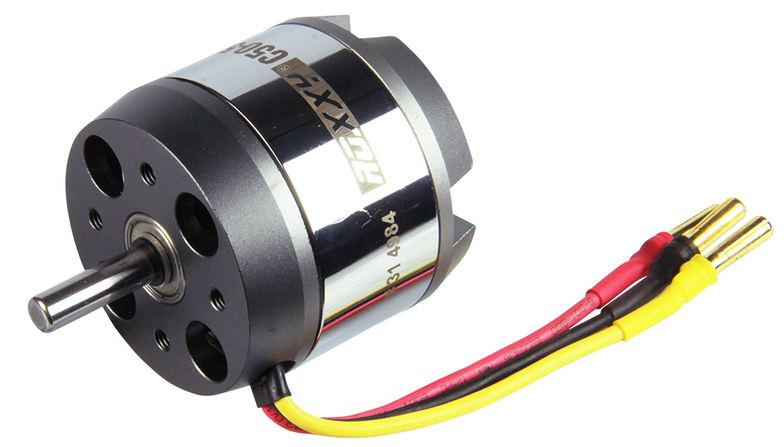
\includegraphics[width=0.6\textwidth]{images/Motor.jpg}
	\caption{Roxxy BL Outrunner C50-55-45 (100KV) \newline (Quelle: mhm-modellbau.de )}
	\label{Motor Roxxy}
\end{figure}

Drehmomentstarker, langsamdrehender Brushless-Elektromotor zum Antrieb großer Schiffs- oder U-Boot-Modelle und Segway-Roboter.

Anzahl : 2x

\textbf{Technische Daten:} 

\begin{itemize} 
	\item Hersteller: Multiplex 
	\item Typ: Outrunner
	\item Nenndrehzahl [kv]: 100
	\item Min. Betriebsspannung [V]: 10,0
	\item Max. Betriebsspannung [V]: 12,6
	\item Dauerstrom [A]: 16,0
	\item Gewicht [g]: 290,0
\end{itemize}

\newpage

\subsection{Endcoder}

\begin{figure}[htb]
	\centering
	\begin{minipage}{0.38\linewidth}
		\centering
		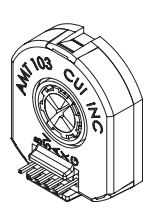
\includegraphics[scale=0.9]{images/Entcoder.jpg}
		\caption{AMT103-V  \newline (Quelle: cui.com)}
		\label{Endcoder}
	\end{minipage}
	\begin{minipage}[h]{0.6\textwidth}
		\textbf{Technische Daten:} 
		\begin{itemize} 
			\item Hersteller: CUI Inc.
			\item Modell:	AMT103-V
			\item Status der Komponente:	Aktiv
			\item Encodertyp:	Kapazitiv
			\item Ausgabetyp: Quadratur mit Index (inkremental)
			\item Impuls pro Umdrehung: Programmierbar
			\item Spannungsversorgung:	3,6 V bis 5,5 V
		\end{itemize}
	\end{minipage}
\end{figure}


\subsection{oDriver}

\begin{figure}[htb]
	\centering
	\begin{minipage}{0.38\linewidth}
		\centering
		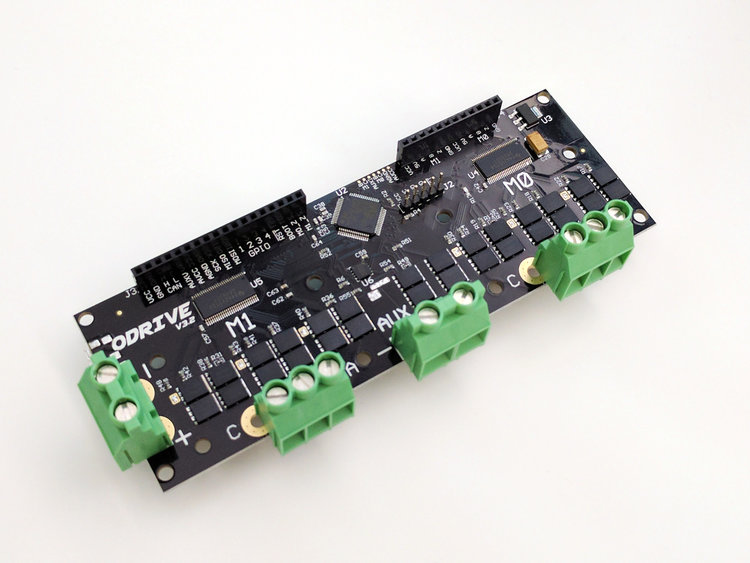
\includegraphics[scale=0.2]{images/odrive.jpeg}
		\caption{oDrive-Platine  \newline (Quelle: https://odriverobotics.com)}
		\label{odrive}
	\end{minipage}
 \begin{minipage}[h]{0.6\textwidth}
	\textbf{Technische Daten:} 
	\begin{itemize} 
		\item Zwei Motorkanäle
		\item 24V, für mehr als 100 A Spitzenstrom ausgelegt.
		\item DC-DC-Wandler für den Bremswiderstand oder Energiespeicherung.
		\item Geberrückführung für beliebig präzise Bewegungen.
		
	\end{itemize}
\end{minipage}
\end{figure}

\begin{itemize} 
\item Unterstützt Leistungsregeneration.
\item Optional Verwendung einer hohe Leistungsdichte Batterie bedeutet, dass Sie erreichen können,> 1 kW Spitzenleistung mit nur einer bescheidenen Stromversorgung.
\item Open Source: Hardware , Software
\item Anschlüsse: USB Serial Port, CAN, UART, PWM
\item Schritt / Richtung - Bestehende Bewegungssteuerungen
\item Einige allgemeine digitale und analoge Stifte
\item PROTOKOLLE: Viele Arten von Befehlsarten, 
Goto (Lageregelung mit Bahnplanung), 
Positionsbefehle, 
Geschwindigkeitsbefehl, 
Drehmomentbefehl.
\end{itemize}

\subsection{Steuerungsplatine}


\begin{figure}[!h]  % [h] bedeutet, dass das Bild genau an dieser Stelle im Text erscheint

	\centering\includegraphics[width=0.7\textwidth]{images/nucleo.jpg}
	\caption{Nucleo-F746ZG  \newline (Quelle: playmbedded.org)}
	\label{Nucleo}
	
\end{figure}


\textbf{Technische Daten:} 

\begin{itemize} 
	\item Mikrocontroller mit 1 MB Flash-Speicher, 320 KB SRAM, mit 216 MHz Cortex-M7-Kern STM32F746ZGT6U
	\item Adaptiver Echtzeitbeschleuniger (ART Accelerator™), der eine 0-Wartezeit-Umsetzung vom Flash-Speicher ermöglicht
	\item LCD-TFT-Controller bis XGA-Auflösung mit dediziertem Chrom-ART Accelerator™
	\item Parallele Kameraschnittstelle, 8–14 Bit, bis zu 54 MB/s
	\item Voller Zugriff auf alle GPIO mit ST Zio-Steckverbinder (Konnektivitätsunterstützung Arduino Uno v3)
	\item ST Morpho-Verlängerungsstiftleiste für den Zugriff auf alle GPIO
	\item ST-LINK/V2-1-Debugger/Programmiergerät mit SWD-Steckverbinder
	\item Bis zu 25 serielle Kommunikationsschnittstellen: USART, IrDA, I²C, SPI, LIN, CAN, USB, I²S, SDIO, HDMI-CEC, S/PDIF-Rx, Ethernet
	\item Flexibles Platinen-Netzteil
	\item USB OTG oder FS-Einheit mit micro-AB-Steckverbinder
	\item Echter Zufallszahlgenerator
	\item CRC-Kalkulationseinheit
	\item RTC mit einer Genauigkeit eines Sekundenbruchteils und Hardware-Kalender
	\item Eindeutige 96-Bit-ID
	\item Drei LEDs: Power-LED, USB-Verbindung, Benutzer-LED
	\item Benutzer- und Reset-Drucktasten
	\item Quarzoszillator, 32,768 KHz
	\item ARM mbed-fähig (mbed.org)
	
\end{itemize}


\subsection{Die Räder}

Es wurden die Reifen bestellt und die Felgen über selbst-erzeugte 3D-Modell gesintert.

\begin{figure}[htb]
	\centering
	\begin{minipage}{0.45\linewidth}
		\centering
		\includegraphics[scale=0.5]{images/reifen.png}
		\caption{Felgen \newline (Quelle: Eigene Darstellung)}
	\end{minipage}
	%\hfill
	\begin{minipage}{0.45\linewidth}
		\centering
		\includegraphics[scale=0.5]{images/reifen.png}
		\caption{Felgen \newline (Quelle: Eigene Darstellung)}
	\end{minipage}
\end{figure}


\begin{figure}[htb]
	\centering
	\begin{minipage}{0.4\linewidth}
		\textbf{Technische Daten:} 
		\begin{itemize} 
			\item TAMIYA DB-01 Dual Block Reifen "C" hinten 62/35 Tuningversion
			\item RC-Maßstab:  1:10 OffRoad
			\item Reifendurchmesser: 87mm
			\item Reifenbreite: 43mm
			\item Modellbauartikel - kein Spielzeug!
		\end{itemize}
	\end{minipage}
	\begin{minipage}[h]{0.4\textwidth}
		\textbf{Technische Daten:} 
		\begin{itemize} 
			\item Material:
			\item 
			\item 
			\item 
			\item 
			\item 
			\item 
		\end{itemize}
	\end{minipage}
\end{figure}

Reifen-Quelle:
https://www.haertle.de/RC+Modellbau/RC+Car+Zubehoer/Reifen+Felgen+Raeder/TAMIYA+54188+DB+01+Dual+Block+Reifen+C+hinten+62+35.html


\subsection{Die Hinderniserkenner}

\begin{figure}[htb]
	\centering
	\begin{minipage}{0.45\linewidth}
		\centering
		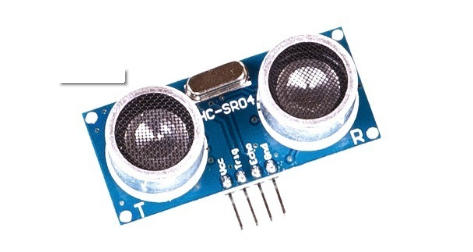
\includegraphics[scale=0.5]{images/Bild-1-1.png}
		\caption{Ultraschallsensor \newline(Quelle: funduinoshop.com)}
		\label{bild_1.2}
	\end{minipage}
	%\hfill
	\begin{minipage}{0.45\linewidth}
		\centering
		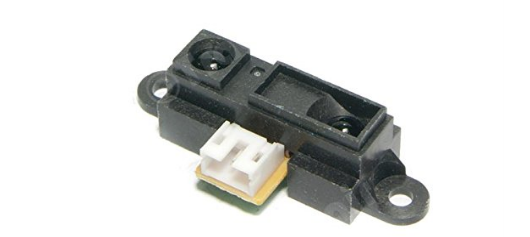
\includegraphics[scale=0.5]{images/infrarot.png}
		\caption{Infrarot-Sensor \newline (Quelle: ebay.de)}
	\end{minipage}
\end{figure}
US-Sensor und Infrarot-Sensor

\begin{figure}[htb]
	\centering
	\begin{minipage}{0.45\linewidth}
		\textbf{Technische Daten:} 
		\begin{itemize} 
			\item 	
			\item 	
			\item 	
			\item 	
			\item 	Erkennen von Umfang: 2cm-4,5 m 
			\item 	Hohe Genauigkeit: bis zu 0,3 cm
			\item 	Sensorwel: Nicht mehr als 15 Grad
			\item 	Versorgungsspannung: DC 5V
			\item Stromverbrauch: 15mA		
			\item Modus der Verbindung: VCC, trig(T), echo(R), 4. GND		
			\item Masse: 4.6 x 2 x 1,3 cm
		\end{itemize}
	\end{minipage}
	\begin{minipage}[h]{0.45\textwidth}
		\textbf{Technische Daten:} 
		\begin{itemize} 
			\item SHARP IR-GP2Y0A21YK0F Distanz Sensor
			\item Einfache Verwendung durch Mikrocontroller, so wie Arduino , 8051, AVR, PIC, DSP, ARM, MSP430, PLC,TTL-Logik
			\item Abstandsmessbereich 10cm – 80cm
			\item Betriebsspannung 5V DC
			\item Stromaufnahme 40 mA
			\item Sensorausgang: alnaloge Spannung
			\item Ausgangsspannung: ca. 0.4V bei 80cm, ca. 2.3V bei 10cm
			\item Ansprechzeit: 39ms
			\item Abmessung: 29,5*13*13,5mm
			
		\end{itemize}
	\end{minipage}
\end{figure}

\newpage

\subsection{Bewegungs- und Beschleunigungsaufnehmer }

Hyroskop Modul-Name und Bild

\subsection{Netz (Akku)}

 Name und Bild
 
 \subsection{...}
 
 Name und Bild

